\documentclass[border=10pt]{standalone}

\usepackage{tikz}
\usepackage{tikzsymbols}
\usetikzlibrary{calc,patterns,shapes.geometric}

\def\centerarc[#1](#2)(#3:#4:#5){\draw[#1] ($(#2)+({#5*cos(#3)},{#5*sin(#3)})$) arc (#3:#4:#5);}

\begin{document}
	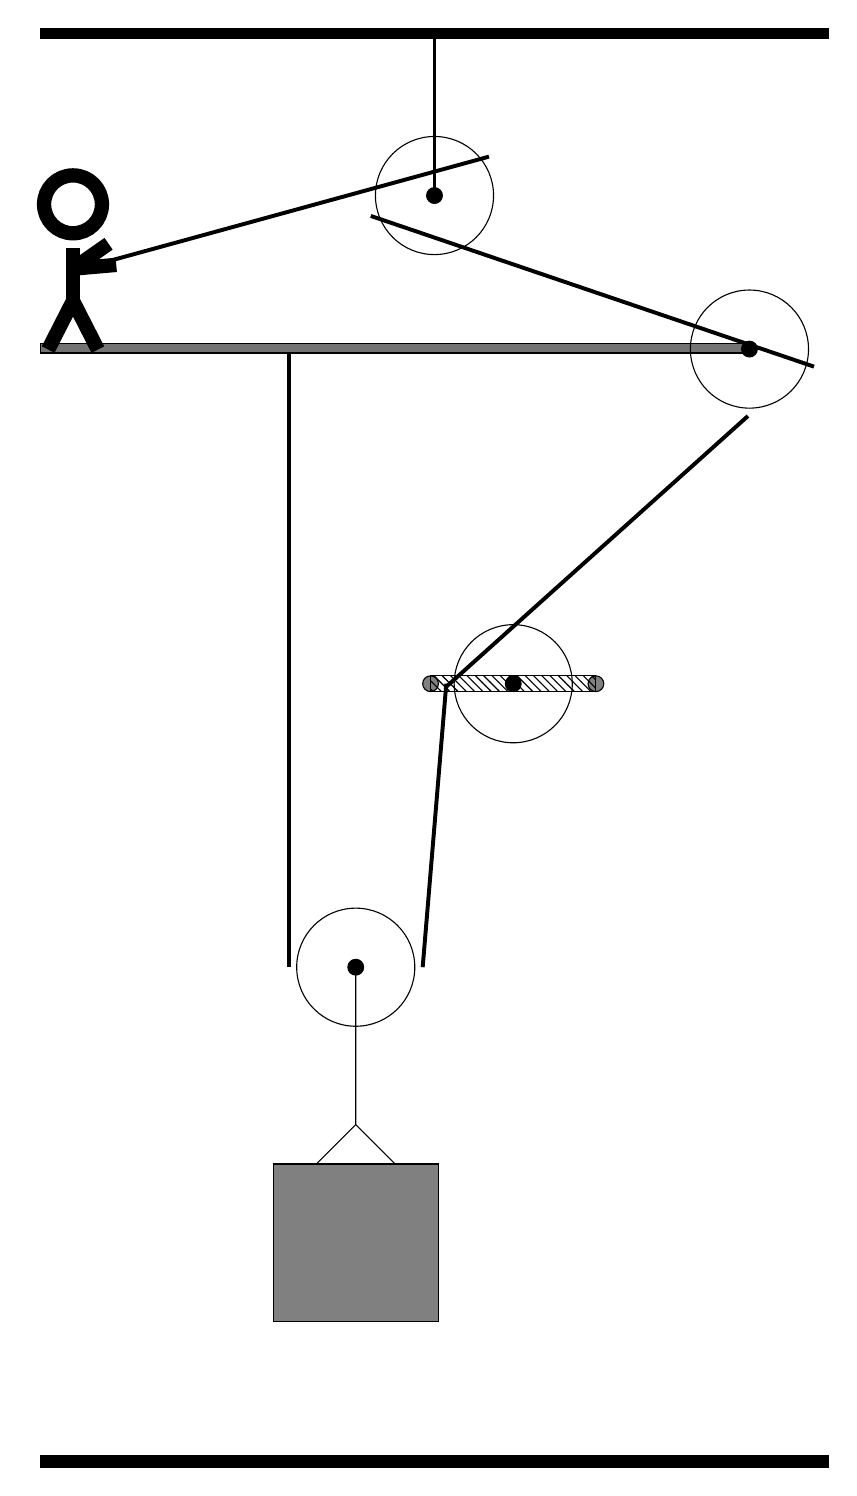
\begin{tikzpicture}
		%%%%% START %%%%%
		\draw[fill=black] (-2, 16) rectangle (8, 16.125);
		
		\draw[fill=black!55] (-2, 12) rectangle (7, 12.125);
		
		\draw (2, 4.2) circle (0.75);
		\draw[fill=black] (2, 4.2) circle (0.1);
		
		\draw (7, 12.05) circle (0.75);
		\draw[fill=black] (7, 12.05) circle (0.1);
		
		\draw[fill=white](4, 7.8) circle (0.75);
		\draw[fill=black] (4, 7.8) circle (0.1);
		\draw[fill=black!50] (2.95, 7.8) circle (0.1);
		\draw[fill=black!50] (5.05, 7.8) circle (0.1);
		\draw[pattern=north west lines, pattern color=black] (2.95, 7.9) rectangle (5.05, 7.7);
		
		\draw (3, 14) circle (0.75);
		\draw[fill=black] (3, 14) circle (0.1);
		\draw[line width=0.5mm] (3, 14) -- (3, 16);
		
		\draw (2, 4.2) -- (2, 2.2) -- (1.5, 1.7) -- (2.5, 1.7) -- (2, 2.2);
		\draw[fill=black!50] (0.95, 1.7) rectangle (3.05, -0.3);
		
		\draw[line width=0.5mm] (1.15, 12) -- (1.15, 4.2);
		\centerarc[line width=0.5mm](2, 4.2)(180:360:0.85);
		\draw[line width=0.5mm](2.85, 4.2) -- (3.15, 7.8);
		\centerarc[line width=0.5mm](4, 7.8)(110:180:0.85);
		\draw[line width=0.5mm](3.151, 7.763) -- (6.981, 11.2);
		\centerarc[line width=0.5mm](7, 12.05)(-60:50:0.85);
		\draw[line width=0.5mm](7.82, 11.827) -- (2.191, 13.741);
		\centerarc[line width=0.5mm](3, 14)(60:120:0.85);
		\draw[line width=0.5mm](3.692, 14.494) -- (-1.2, 13.15);
		
		\node at (-1.5, 13.15) {\Strichmaxerl[10][-175][35]};
		
		\draw[fill=black] (-2, -2) rectangle (8, -2.15);
		%%%%% END %%%%%
	\end{tikzpicture}
\end{document}